\chapter{Dualità}
La dualità permette di associare a un problema di programmazione lineare detto \textbf{primale}:
\[min(c^Tx) \quad Ax \geq b \quad x \geq 0\]  
Un altro problema di programmazione lineare detto \textbf{duale}
\[max(y^Tb) \quad y^TA\leq c^T \quad y \geq 0\] 
\\Questo permette di avere alcuni vantaggi:
\begin{enumerate}
    \item \textbf{Risolutivi}: il duale può essere più facile da risolvere rispetto al problema primale. 
    \item \textbf{Interpretativo}: il significato economico del primale si può evincere meglio dal problema duale.
    \item \textbf{Algoritmico}: si utilizza il metodo del simplesso duale.
    \item \textbf{ Analisi post-ottimale.}
\end{enumerate}

Per passare da un problema all'altro è possibile seguire specifiche regole così definite:
\begin{figure}[H]
    \centering
    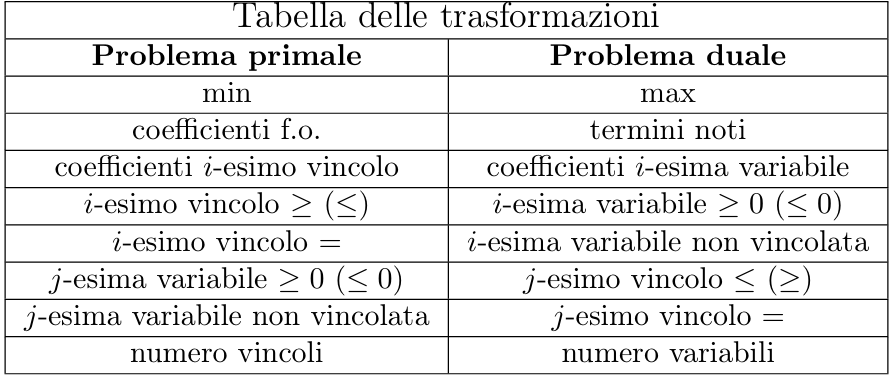
\includegraphics[width=0.7\linewidth]{Images/dualita/tabella_trasformazioni.png}
\end{figure}
È bene segnalare che, questa tabella non deve essere necessariamente letta da sinistra verso destra, cioè da problema di minimo a problema di massimo, ma anche da problema di massimo a problema di minimo stando attenti a ricordare che le regole non sono uguali in ambo i casi.
Possiamo schematizzarle in maniera semplice così:
\begin{figure}[H]
    \centering
    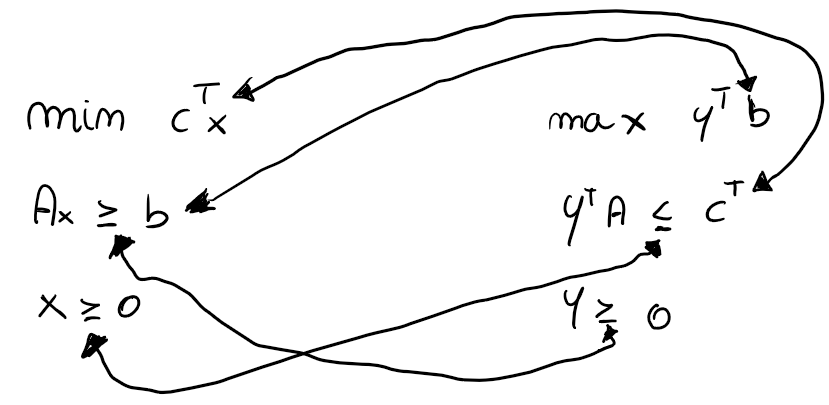
\includegraphics[width=0.4\linewidth]{Images/dualita/schema_trasformazioni.png}
\end{figure}
Guardiamo un esempio di come avviene questo processo:
\begin{figure}[H]
    \centering
    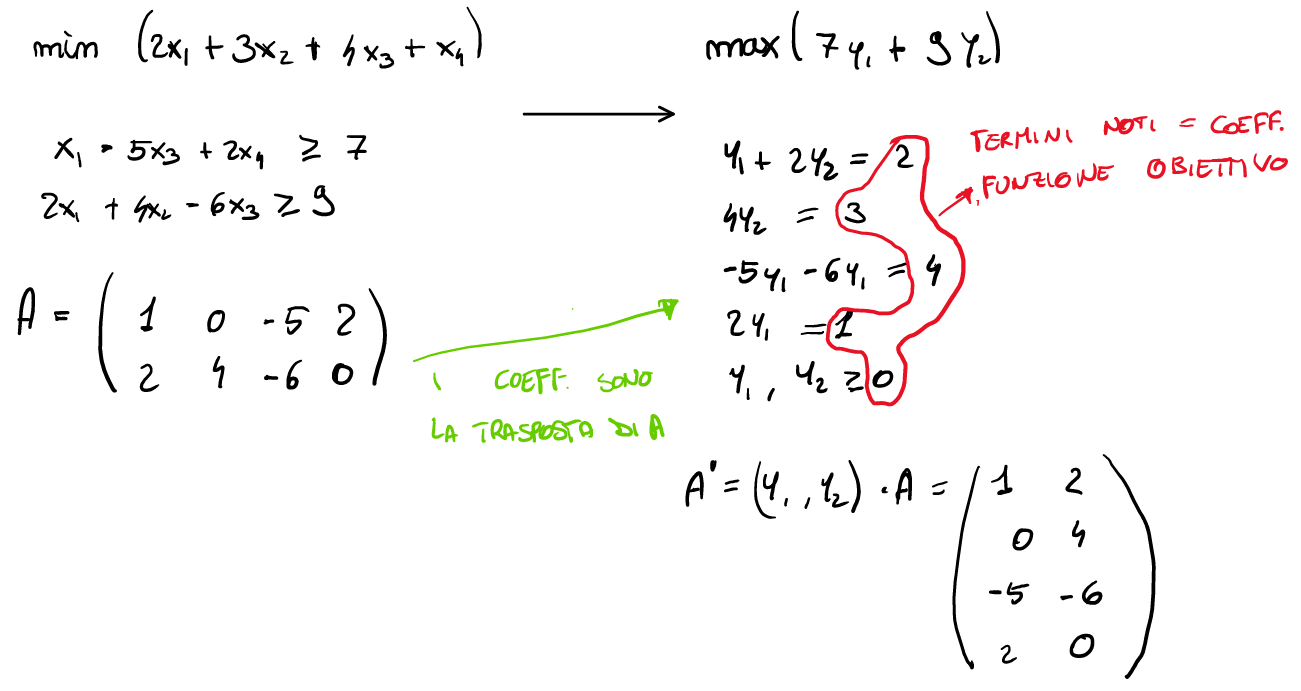
\includegraphics[width=0.8\linewidth]{Images/dualita/esempio_1_trasformazione.png}
\end{figure}

Chiamiamo problemi duali \textbf{simmetrici} i problemi di programmazione lineare con la seguente forma:
\begin{align*}
    &\min (c^Tx) \xrightarrow{} \max (y^Tb)\\
    &Ax \geq b \xrightarrow{} y^TA \leq c^T\\
    &x \geq 0 \xrightarrow{} y \geq 0
\end{align*}
\begin{figure}[H]
    \centering
    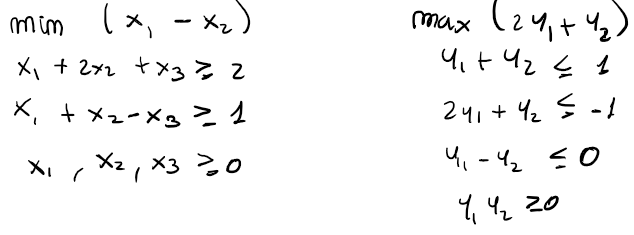
\includegraphics[width=0.8\linewidth]{Images/dualita/duale_simmetrico.png}
\end{figure}

Chiamiamo, invece, problemi duali \textbf{anti-simmetrici} i problemi per cui i primali sono in forma standard e, quindi:
\begin{align*}
    &\min(c^Tx) \xrightarrow{}\max(y^Tb)\\
    &Ax=b \xrightarrow{} y^TA \leq c^T\\
    &x \geq 0 \xrightarrow{} ///
\end{align*}
\begin{figure}[H]
    \centering
    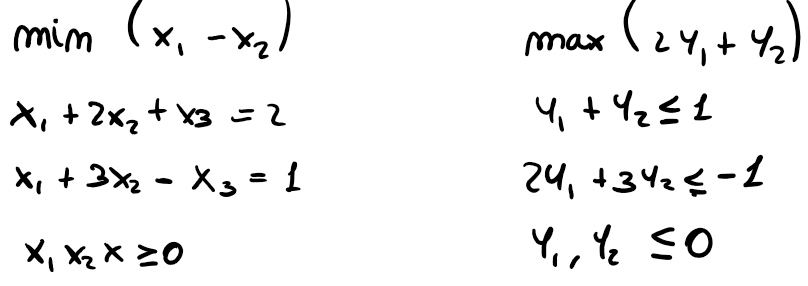
\includegraphics[width=0.8\linewidth]{Images/dualita/duale_asimmetrico.png}
\end{figure}
\section{Teorema di dualità debole}
Sia $x'$ una soluzione ammissibile del problema primale di $min(c^Tx) \quad  Ax \geq b \quad x \geq 0$ e sia $y'$ una
soluzione ammissibile del duale $max (y^Tb)\quad y^TA \leq c^T\quad y \geq 0$, allora $y'^T b \leq c^T x'$.

Se prendiamo la soluzione ottima del problema duale, abbiamo un lower bound per il problema primale:
\[y' = y^{ott} \quad (y^{ott})b \leq c^Tx'\]
Allo stesso modo,  la soluzione ottima del primale è upper bound del problema duale.
\[x' = x^{ott} \quad y'^Tb \leq c^Tx^{ott}\]
Inoltre, se abbiamo una soluzione per uno dei due problemi, allora abbiamo una soluzione anche per l'altro.

\textbf{Corollario criterio di ottimalità}
Sia $x'$ ammissibile per il problema primale e sia $y'$ ammissibile per il problema duale, se $y'^Tb = c^T x'$, allora $x',y'$ sono ottimi per i rispettivi problemi. 
Inoltre, se uno dei due problemi primali o duale è illimitato, l'altro è inammissibile.

\section{Teorema della dualità forte}
Se uno dei due problemi primale o duale ammette soluzione ottima finita, anche l’altro ha una soluzione ottima finita e i corrispondenti valori delle funzioni obiettivo coincidono. Se uno dei due problemi è illimitato, l’altro non ammette soluzioni ammissibili
\begin{figure}[H]
    \centering
    
\includegraphics[width=0.5\linewidth]{Images/dualita/tabella_pd.png}
\end{figure}
\section{Teorema degli scarti complementari}
Siano $x'$ ed $y'$ soluzioni ammissibili rispettivamente per il primale e per il duale. Allora $x'$ e $y'$ sono soluzioni ottime per i rispettivi problemi se e solo se soddisfano le condizioni di complementarietà:
\begin{equation*}
    \begin{cases}
        y'^T(Ax-b) = 0\\
        (y^TA-c^T)x' = 0 \\
    \end{cases}
\end{equation*}
\begin{figure}[H]
    \centering
    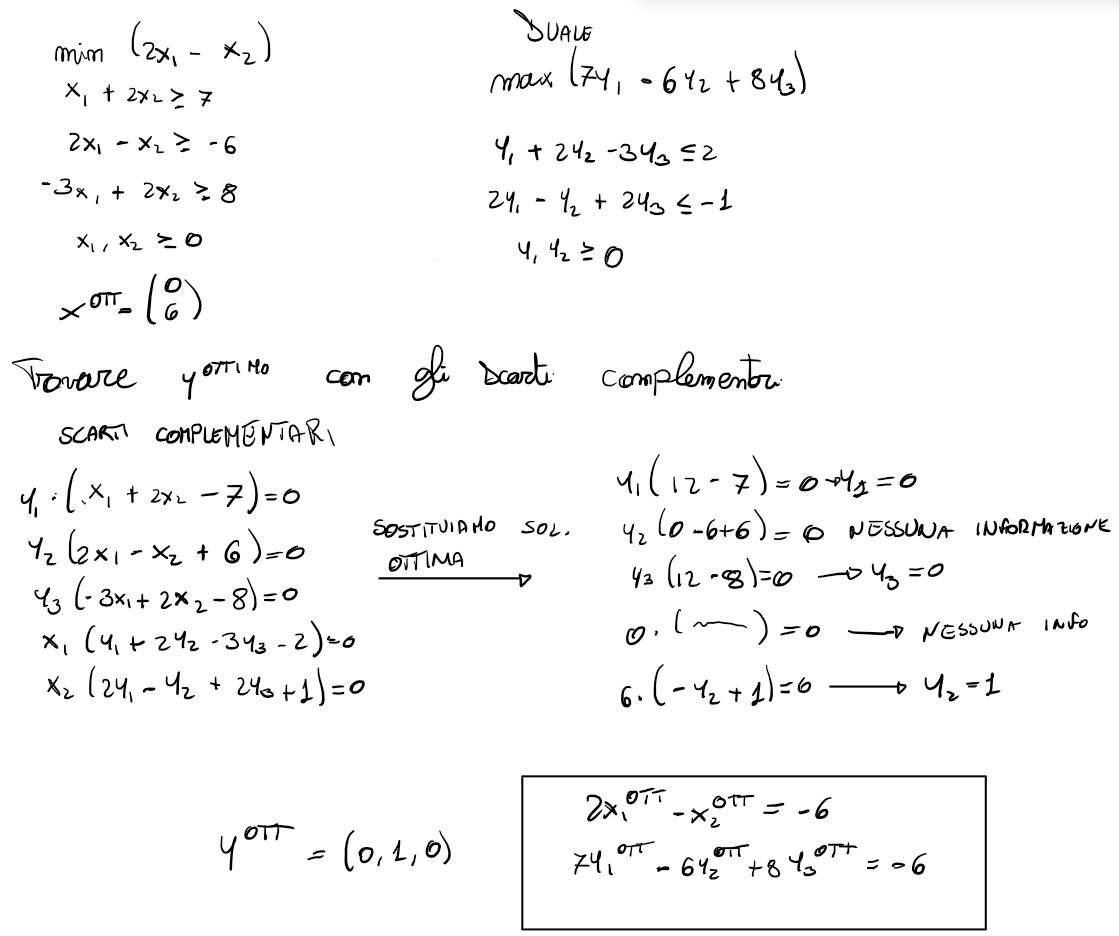
\includegraphics[width=1\linewidth]{Images/dualita/esempio_scarti_complementari.png}
\end{figure}
\section{Calcolo della soluzione ottimale}
La soluzione ottima del duale può essere ottenuta direttamente dalla tabella finale del problema
primale. Se il primario ha solo vincoli $\leq$, allora possiamo calcolare la soluzione ottimale del duale come 
\begin{align*}
    &\text{coefficienti della funzione obiettivo delle variabili in base alla prima iterazione} -\\
    &\text{costi ridotti delle variabili in base alla prima iterazione letti nella tabella finale}
\end{align*}

\begin{figure}[H]
    \centering
    
\includegraphics[width=0.8\linewidth]{Images/dualita/esempio_complementari/1.png}
\end{figure}
Il duale diventa:
\begin{figure}[H]
    \centering
    
\includegraphics[width=1\linewidth]{Images/dualita/esempio_complementari/2.png}
\end{figure}

Esiste un altro modo per calcolare la soluzione ottima del duale che consiste nell'effettuare il prodotto riga per colonna tra i coefficienti della funzione obiettivo delle componenti in base della soluzione di base ottima finale per la matrice che ha per colonne le variabili di base della prima iterazione nell'ultima tabella. Applicato all'esempio precedente:
\begin{figure}[H]
    \centering
    
\includegraphics[width=1\linewidth]{Images/dualita/esempio_complementari/3.png}
\end{figure}

\section{Interpretazione della dualità}
Cerchiamo adesso di capire cosa ci va' a dire, in contesti reali, il duale di alcuni dei problemi che abbiamo già affrontato.
\subsection{Problema dei mattoncini lego}
Dato il problema:
\[\max(15x_1+20x_2) \quad x_1+2x_2\leq 6 \quad 2x_1+2x_2 \leq 8 \quad x_1,x_2 \geq
0\]

Considereremo il duale come una sorta di mercato parallelo detto \textbf{mercato ombra} in cui si  vendono le materie prime e si vogliono determinare i prezzi di vendita $y_1$ di mattoni grandi e $y_2$ mattoni piccoli in modo da associare a essi valori più bassi possibili per rendere la loro vendita competitiva. L'obiettivo sarà rendere $\min(6y_1+8y_2)$ con i vincoli per cui vogliamo che il profitto della vendita dei mattoni per una sedia o per un tavolo dovrà essere $\geq$ del profitto della vendita della sedia o del tavolo,  diversamente non sarebbe conveniente vendere le materie prime. Per cui i vincoli saranno:

\begin{align*}
    &y_1+2y_2 \geq 15\\
    &2y_1+2y_2 \geq 8\\
    &y_1,y_2 \geq 0
\end{align*}

Che corrispondono esattamente al duale del problema iniziale. Se parliamo di variabili complementari avremo che:
\begin{align*}
    &y_1(x_1+2x_2-6)=0\\
    &y_2(2x_1+2x_2 - 8) = 0\\ 
\end{align*}

Da queste relazioni deduciamo che: 
\begin{itemize}
    \item se $x_1+2x_2 < 6$ allora avremo che $y_1 = 0 \xrightarrow{}$ vuol dire che non stiamo utilizzando tutti i 6 mattoni, allora il prezzo ombra deve essere zero poiché non ha senso comprare altri mattoni.
    \item Se $y_1 > 0$, allora $x_1+2x_2 = 6$ vale il contrario di quanto detto prima, cioè stiamo utilizzando tutti i mattoni per cui potrebbe essere conveniente comprarne altri.
\end{itemize}
In un certo senso le variabili complementari ci dicono come cambia il profitto della funzione obiettivo primaria se incremento di una unità la scorta.

\subsection{Duale della dieta ottimale}
Preso il problema della dieta ottimale: 
\[\min(c^Tx) \quad Ax \geq b \quad x \geq 0\] 
Diventa: 
\[\max(y^Tb) \quad y^TA \leq c^T \quad y \geq 0\]

Il duale considera la vendita dei principi nutritivi piuttosto ché la vendita del cibo.\footnote{Sarà come considerare le vendite di un'azienda che vende integratori}
Nel problema duale si determinano i prezzi di vendita dei principi nutritivi in modo da massimizzare il profitto. Per rendere competitiva l'operazione, il prezzo dei principi nutritivi di ogni alimento deve essere $\leq$ del prezzo dell'alimento originale.

\subsection{Duale del problema del trasporto}
Dati m magazzini e n depositi, si vuole minimizzare il prezzo di trasporto di un prodotto dal magazzino i al magazzino j in modo da rispettare i vincoli sull'offerta di p e sulla domanda di j. Avremo quindi:
\begin{align*}
    &\min (\sum_i^m \sum_j c_{ij} x_{ij}) \text{costo di trasporto da i a j.}\\
    &\sum_j x_{ij} = p_i \text{vincoli sull'offerta/ disponibilità del prodotto}\\
    &\sum_i x_{ij} = q_j \text{vincoli sulla domanda}
    x_{ij} \geq 0 
\end{align*}

Il duale rappresenta una piccola compagnia si propone di prelevare 1 unità di prodotto dal magazzino con il prezzo $u_i$ e di consegnarla al deposito j al prezzo $v_j$.
Dovrà essere conveniente per l'azienda di trasporto del problema primario. Ne segue che $u_i+v_j \leq c_{ij}$.
La piccola compagnia vuole massimizzare il profitto, per cui avremo che:
\begin{align*}
    &Max(\sum_i^m p_iu_i+\sum_j^n q_jv_j)\\
    &u_i+v_j \leq c_{ij} \forall i, j
\end{align*}

\section{Simplesso duale}
Consideriamo un generico problema duale per cui avremo il problema primale:
\[min(c^Tx) \quad Ax \geq b \quad x \geq 0\]  
E il rispettivo problema duale:
\[max(y^Tb) \quad y^TA\leq c^T \quad y \geq 0\] 

\textbf{La condizione di ammissibilità duale è la condizione di ottimalità primale}\\
Ricordiamoci che per il teorema della dualità forte, vale che: 
\[y'^Tb = c^Tx'\]

Che possiamo anche riscrivere come: 
\[y'^Tb= c_B^T x'_B+c_N^T x'_N\]\\
Se $x'$ è soluzione ottima del problema primale, allora avremo che $ x'_B = B^{-1}b, x'_N = (0, \dots, 0)$, per cui:
\[y'^Tb= c_B^T x'_B+c_N^T x'_N = c^T_B B^{-1}b\]

Ora alla base B possiamo associare la soluzione $y_B^T = c_B^T B^{-1}$ che deve essere ammissibile per il duale, per cui abbiamo bisogno che:
\begin{align*}
    &y_B^TB\leq c_B^T\\
    &y_B^TN\leq c_N^T
\end{align*}
\begin{figure}[H]
    \centering
    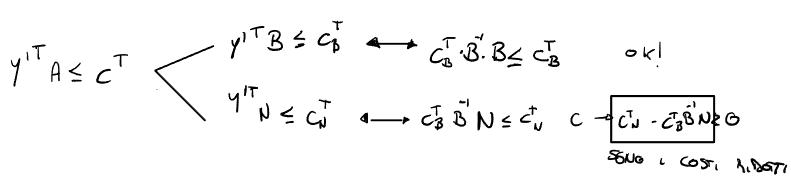
\includegraphics[width=0.8\linewidth]{Images/dualita/condizione_ammissibile_primale_duale.png}
\end{figure}

Per cui, la condizione di ammissibilità duale ($c_N^T - c_B^T B^{-1}N \geq 0$) coincide con l'ottimalità primale ($costi-ridotti \geq 0$).

Il metodo del simplesso duale si applica per risolvere il primale quando ci sono termini noti negativi, cioè, manca l'ammissibilità primale, ma abbiamo l'ammissione duale, cioè abbiamo costi ridotti positivi. Dal punto di vista geometrico è come se partissimo da dei vertici al di fuori della regione ammissibile e cerchiamo di raggiungere i vertici ottimi da lì.

\textbf{Criterio di uscita e di entrata}\\
Anche in questo caso considereremo un criterio di uscita e di entrata in base per cui guardiamo la riga dove troviamo un termine noto negativo e consideriamo gli elementi della riga $\alpha_{rj}$: 
\begin{enumerate}
    \item Se tutti gli $\alpha_{rj} \geq 0 \quad \forall j$, allora il problema è \textbf{inammissibile}.
    \item Se abbiamo $\alpha_{rj} \leq 0$ allora cambiamo base ed esce $x_r$ corrispondente alla riga del termine noto negativo, e facciamo entrare in base:
    \[\min(\frac{r_j}{|\alpha_{rj|}}:\alpha_{rj}<0)\]
    Dove $\alpha_{rj}$ è il \textbf{pivot} delle operazioni.
\end{enumerate}
Vediamo un esempio di come applicare questo metodo:
\begin{figure}[H]
    \centering
    
\includegraphics[width=1\linewidth]{Images/dualita/esempio_simplesso_duale/1.png}
\end{figure}
\begin{figure}[H]
    \centering
    
\includegraphics[width=1\linewidth]{Images/dualita/esempio_simplesso_duale/2.png}
\end{figure}
\begin{figure}[H]
    \centering
    
\includegraphics[width=1\linewidth]{Images/dualita/esempio_simplesso_duale/3.png}
\end{figure}

\section{Analisi Post-Ottimale}
Vediamo come può variare la soluzione ottima del problema 
\[\min c^Tx \quad Ax\geq b \quad x \geq 0\]
perturbando i termini noti o i coefficienti di costo.
\subsection{Perturbazione dei termini noti}
Supponiamo di voler perturbare la componente $b_r$ del vettore dei termini noti del problema iniziale in maniera tale che questo diventi $b_r+\Delta b_r$. Indichiamo con $\bar{b}$ il vettore dei termini noti perturbati. La nuova soluzione ottima primale è $x^T=(B^{-1}\bar{b},0)$.
Possono accadere due cose:
\begin{enumerate}
    \item Se $B^{-1}\bar{b}$ ha delle componenti negative, la soluzione di base primale $\tilde{x}$ non è più ammissibile. Tuttavia, poiché $c_N^T-c_B^T B^{-1}N\geq 0$, la soluzione duale è ancora ammissibile e si può risolvere il problema mediante il simplesso duale. 
    \item Se $B^{-1}\bar{b}\geq 0$ allora $\tilde{x}$ è una SBA. I costi ridotti sono dati da  $c_N^T-c_B^T B^{-1}N$ e sono maggiori di 0 poiché sono gli stessi della soluzione ottima $\bar{x}$. Dunque, anche $\tilde{x}$ è SBA ottima. Per cui, la soluzione ottima duale $y^T =c^T_B B^{-1}$ resta la stessa sia nel problema iniziale che nel problema duale.
\end{enumerate}
Vediamo come varia la funzione obiettivo in relazione alle due soluzioni $\bar{x}(c^T\bar{x})$ e $\tilde{x}(c^T\tilde{x})$.

\begin{align*}
    &c^T\bar{x}-c^T\tilde{x}=c^T_B\bar{x_B}+c^T_N\bar{x_N}-c^T_B\tilde{x_B}+c^T_N\tilde{x_N}\\
    &=c^T_B B^{-1}\bar{b}-c^T_B B^{-1}b = \text{ le componenti N sono = 0}\\
    &=\bar{y}^T (\bar{b}-b)= \bar{y_r}\Delta b_r \text{ Dal caso 2, effettuiamo una sostituzione}
\end{align*}

Ne segue quindi che la variabile duale $y_r$ misura la variazione della funzione obiettivo quando si passa da $b_r$ a $b_r+\Delta b_r$.

Vediamo un esempio:
\begin{figure}[H]
    \centering
    
\includegraphics[width=1\linewidth]{Images/dualita/esempio_analisi_post/1.png}
\end{figure}
La variazione della funzione è $y_1 = 0.5$ e il nuovo valore della funzione obiettivo è 9.5.
La variabile duale ci permette di valutare l'incremento del valore della funzione obiettivo senza dover necessariamente risolvere il problema con il termine noto perturbato.
\begin{figure}[H]
    \centering
    
\includegraphics[width=1\linewidth]{Images/dualita/esempio_analisi_post/2.png}
\end{figure}
\begin{figure}[H]
    \centering
    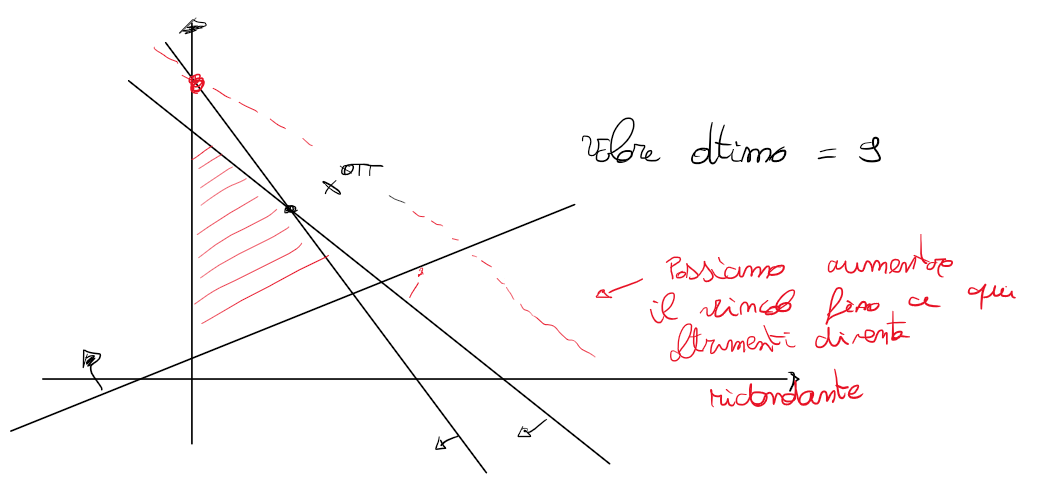
\includegraphics[width=0.7\linewidth]{Images/dualita/esempio_analisi_post/3.png}
\end{figure}